\documentclass[conference]{IEEEtran}
\IEEEoverridecommandlockouts
\usepackage{cite}
\usepackage{amsmath,amssymb,amsfonts}
\usepackage{algorithm}
\usepackage{algorithmic}
\usepackage{graphicx}
\usepackage{textcomp}
\usepackage{xcolor}
\usepackage{placeins}
\usepackage{booktabs}
% Figures live in figs/, alongside this file - self-contained for Overleaf upload.
\graphicspath{{figs/}}
\def\BibTeX{{\rm B\kern-.05em{\sc i\kern-.025em b}\kern-.08em
    T\kern-.1667em\lower.7ex\hbox{E}\kern-.125emX}}
\begin{document}
\raggedbottom

\title{A Multi-Branch AI System for SQL Injection Detection at the Database Proxy with a Zero-Day Generalization Study}

% ==== TODO before submission: fill in [dept/major], [email or ORCID], and Bach's campus city. ====
\author{
\IEEEauthorblockN{1\textsuperscript{st} Bach Luong-Chi}
\IEEEauthorblockA{\textit{School of Science, Engineering \& Technology} \\
\textit{RMIT University Vietnam}\\
{Hanoi}, Vietnam \\
{chibachluong@gmail.com}}
\and
\IEEEauthorblockN{2\textsuperscript{nd} Minh-Duc Do-Xuan}
\IEEEauthorblockA{\textit{International School} \\
\textit{Vietnam National University Hanoi}\\
Hanoi, Vietnam \\
{minhdc42195@gmail.com}}
\and
\IEEEauthorblockN{3\textsuperscript{rd} Diep Dinh-Ngoc}
\IEEEauthorblockA{\textit{ International School} \\
\textit{Vietnam National University Hanoi}\\
Hanoi, Vietnam \\
{dinhngocdiep281104.work@gmail.com}}
\and
\IEEEauthorblockN{4\textsuperscript{th} Minh Nguyen-Quang}
\IEEEauthorblockA{\textit{International School} \\
\textit{Vietnam National University Hanoi}\\
Hanoi, Vietnam \\
{quangminhdang1703@gmail.com}}
\and
\IEEEauthorblockN{5\textsuperscript{th} Linh Dinh-Van}
\IEEEauthorblockA{\textit{[TODO: dept]} \\
\textit{Academy of Cryptography Techniques
}\\
Hanoi, Vietnam \\
{vanlinh@actvn.edu.vn}}
\and
\IEEEauthorblockN{6\textsuperscript{th} Dinh\-Thai Kim}
\IEEEauthorblockA{\textit{International School} \\
\textit{Vietnam National University Hanoi}\\
Hanoi, Vietnam \\
{thaikd@vnu.edu.vn}}
}

\maketitle

\begin{abstract}
SQL Injection (SQLi) remains a damaging web application vulnerability. Signature-based Web Application Firewalls (WAFs) struggle with obfuscated payloads and previously unseen attacks. This paper presents a multi-branch artificial intelligence system for SQLi detection. We position the system at the database proxy to inspect the final SQL statement after application construction but before database execution. The architecture combines a supervised multi-class classifier (Branch 1) and a query-level anomaly detector (Branch 2). Branch 2 trains exclusively on benign traffic. We introduce the Session Correlator to catch blind and multi-step attacks. This mechanism reuses signals from both branches without additional training. On a cleaned public dataset, Branch 1 reaches a 0.9907 F1-macro across five SQLi categories. Branch 2 uses Local Outlier Factor (LOF) to attain a 0.929 Area Under the Curve (AUC). It detects 81.4 percent of anomalous queries at a 5.4 percent false-positive rate (FPR). A zero-day study shows supervised classification remains robust for distinctive attacks but misses Boolean-blind payloads. The anomaly branch independently recovers most of these structural variations. The Session Correlator recovers residual cases on a held-out set of self-generated attack sessions with zero observed false positives. We report this as preliminary evidence pending validation on independently-captured attacker traffic. Finally, we evaluate an offline continual-learning loop. This pipeline uses drift monitoring and a review queue to surface new classes and trigger automatic retraining. These results quantify query-level detection limits and validate session-level correlation.its of query-level detection and motivate session-level correlation and disciplined retraining as low-cost mitigations.
\end{abstract}

\begin{IEEEkeywords}
SQL injection, intrusion detection, anomaly detection, machine learning, web security, zero-day detection
\end{IEEEkeywords}

\section{Introduction}
Web applications store increasingly sensitive data, making their back-end databases a persistent target. SQL Injection (SQLi), in which unsanitized user input is concatenated into a SQL statement, is among the oldest and most severe such threats: successful exploitation can disclose, alter, or destroy data and escalate privileges. Although Web Application Firewalls (WAFs) are widely deployed, rule-based defenses depend on predefined signatures; obfuscated payloads and zero-day techniques bypass them, while overly strict rules raise the false-positive rate (FPR) on legitimate traffic.

Machine learning (ML) and deep learning have emerged as promising alternatives because they learn attack patterns from data rather than from hand-written rules \cite{b1,b2,b3}. However, most published AI-based SQLi detectors classify a \emph{single} query in isolation. This is a structural limitation: Boolean-blind and time-blind SQLi, and query-splitting attacks, distribute their malicious intent across many individually innocuous-looking queries within one session. Their signal only becomes visible when a sequence of related queries is analyzed together.

This paper describes a multi-branch AI system that performs SQLi detection at the \emph{database proxy}, inspecting the fully-built SQL statement before it reaches the database server. Two query-level branches, a supervised multi-class classifier and a benign-only anomaly detector, feed a session-level correlation mechanism that catches blind and multi-step attacks neither branch sees alone. On a combined public dataset, the system reaches an F1-macro of 0.9907 for query-level classification and an AUC of 0.929 for anomaly detection, and a leave-one-out study shows the two branches together recover most attacks that either one misses individually. The contributions of this paper are:

\begin{itemize}
\item A multi-branch detector architecture combining a supervised multi-class classifier (Branch~1) and a benign-only anomaly detector (Branch~2) under a single decision policy, with a session-level correlation mechanism (the Session Correlator) that reuses both branches' existing signals, with no additional training, to catch blind and multi-step SQLi; evaluated with a mandatory ablation over its two constituent checks.
\item A leave-one-out \emph{zero-day} study that quantifies, per attack category, how far each branch generalizes to an attack type it never saw during training, and what this implies for the value of the anomaly branch.
\item An offline evaluation of a continual-learning loop - drift monitoring, a threshold-triggered review queue, and a validation gate with a shadow stage - using a real held-out attack class, with an ablation isolating the retrain gain to the class itself rather than to added data volume.
\end{itemize}

The remainder of the paper reviews related work (Section~\ref{sec:related}), describes the proposed system (Section~\ref{sec:system}) and the experimental setup (Section~\ref{sec:setup}), reports results (Section~\ref{sec:results}), discusses limitations (Section~\ref{sec:discussion}), and concludes (Section~\ref{sec:conclusion}).

\section{Related Work}\label{sec:related}
Traditional SQLi defenses rely on input validation, parameterized queries, and rule-based WAFs such as ModSecurity with the OWASP Core Rule Set. These are fast and interpretable for known attacks but require constant manual updates and are evaded by payload obfuscation \cite{b1}.

ML-based detectors extract features from queries-bag-of-words, Term Frequency-Inverse Document Frequency (TF-IDF), or character/word $n$-grams-and train classifiers such as SVM, Random Forest, or gradient-boosted trees \cite{b2}. Deep models remove the need for handcrafted features: CNNs capture local token patterns \cite{b3}, while recurrent models (LSTM/GRU) and Transformer-based encoders such as DistilBERT model longer-range structure \cite{b5,b6,b7,b8}. For unseen attacks, anomaly and ensemble approaches have been proposed, including autoencoder/LSTM/GRU ensembles for zero-day web attacks \cite{b4}. Classic one-class methods-Isolation Forest \cite{b9} and One-Class SVM \cite{b10}-model the support of the benign distribution and flag deviations, and adversarial tools such as WAF-A-MoLE \cite{b11} expose the fragility of detectors under deliberate evasion.

Across this literature, detection is predominantly \emph{query-level}: a verdict is issued per query. Session-level modeling, which is required to expose blind SQLi spread over many requests, is comparatively underexplored. Our work targets that gap while grounding the design in a measured evaluation of the two query-level branches it builds on.

\section{Proposed System}\label{sec:system}

\subsection{System Placement: The Database Proxy}
The detector is placed at ``Position~B'': it receives the SQL statement after the application has finished constructing it but before the statement reaches the database. Inspecting the final statement (rather than raw HTTP input) removes ambiguity introduced by application-layer transformations and yields a canonical view of what will actually execute. Fig.~\ref{fig:arch} shows the overall flow: each query is canonicalized and scored by Branch~1 and Branch~2; the Session Correlator correlates both branches' signals over a whole session; the decision engine emits ALLOW/BLOCK/OVERKILL. Algorithm~\ref{alg:detect} summarizes the per-query decision.

% TODO: replace this placeholder box with the real architecture diagram.
\begin{figure*}[t]
\centerline{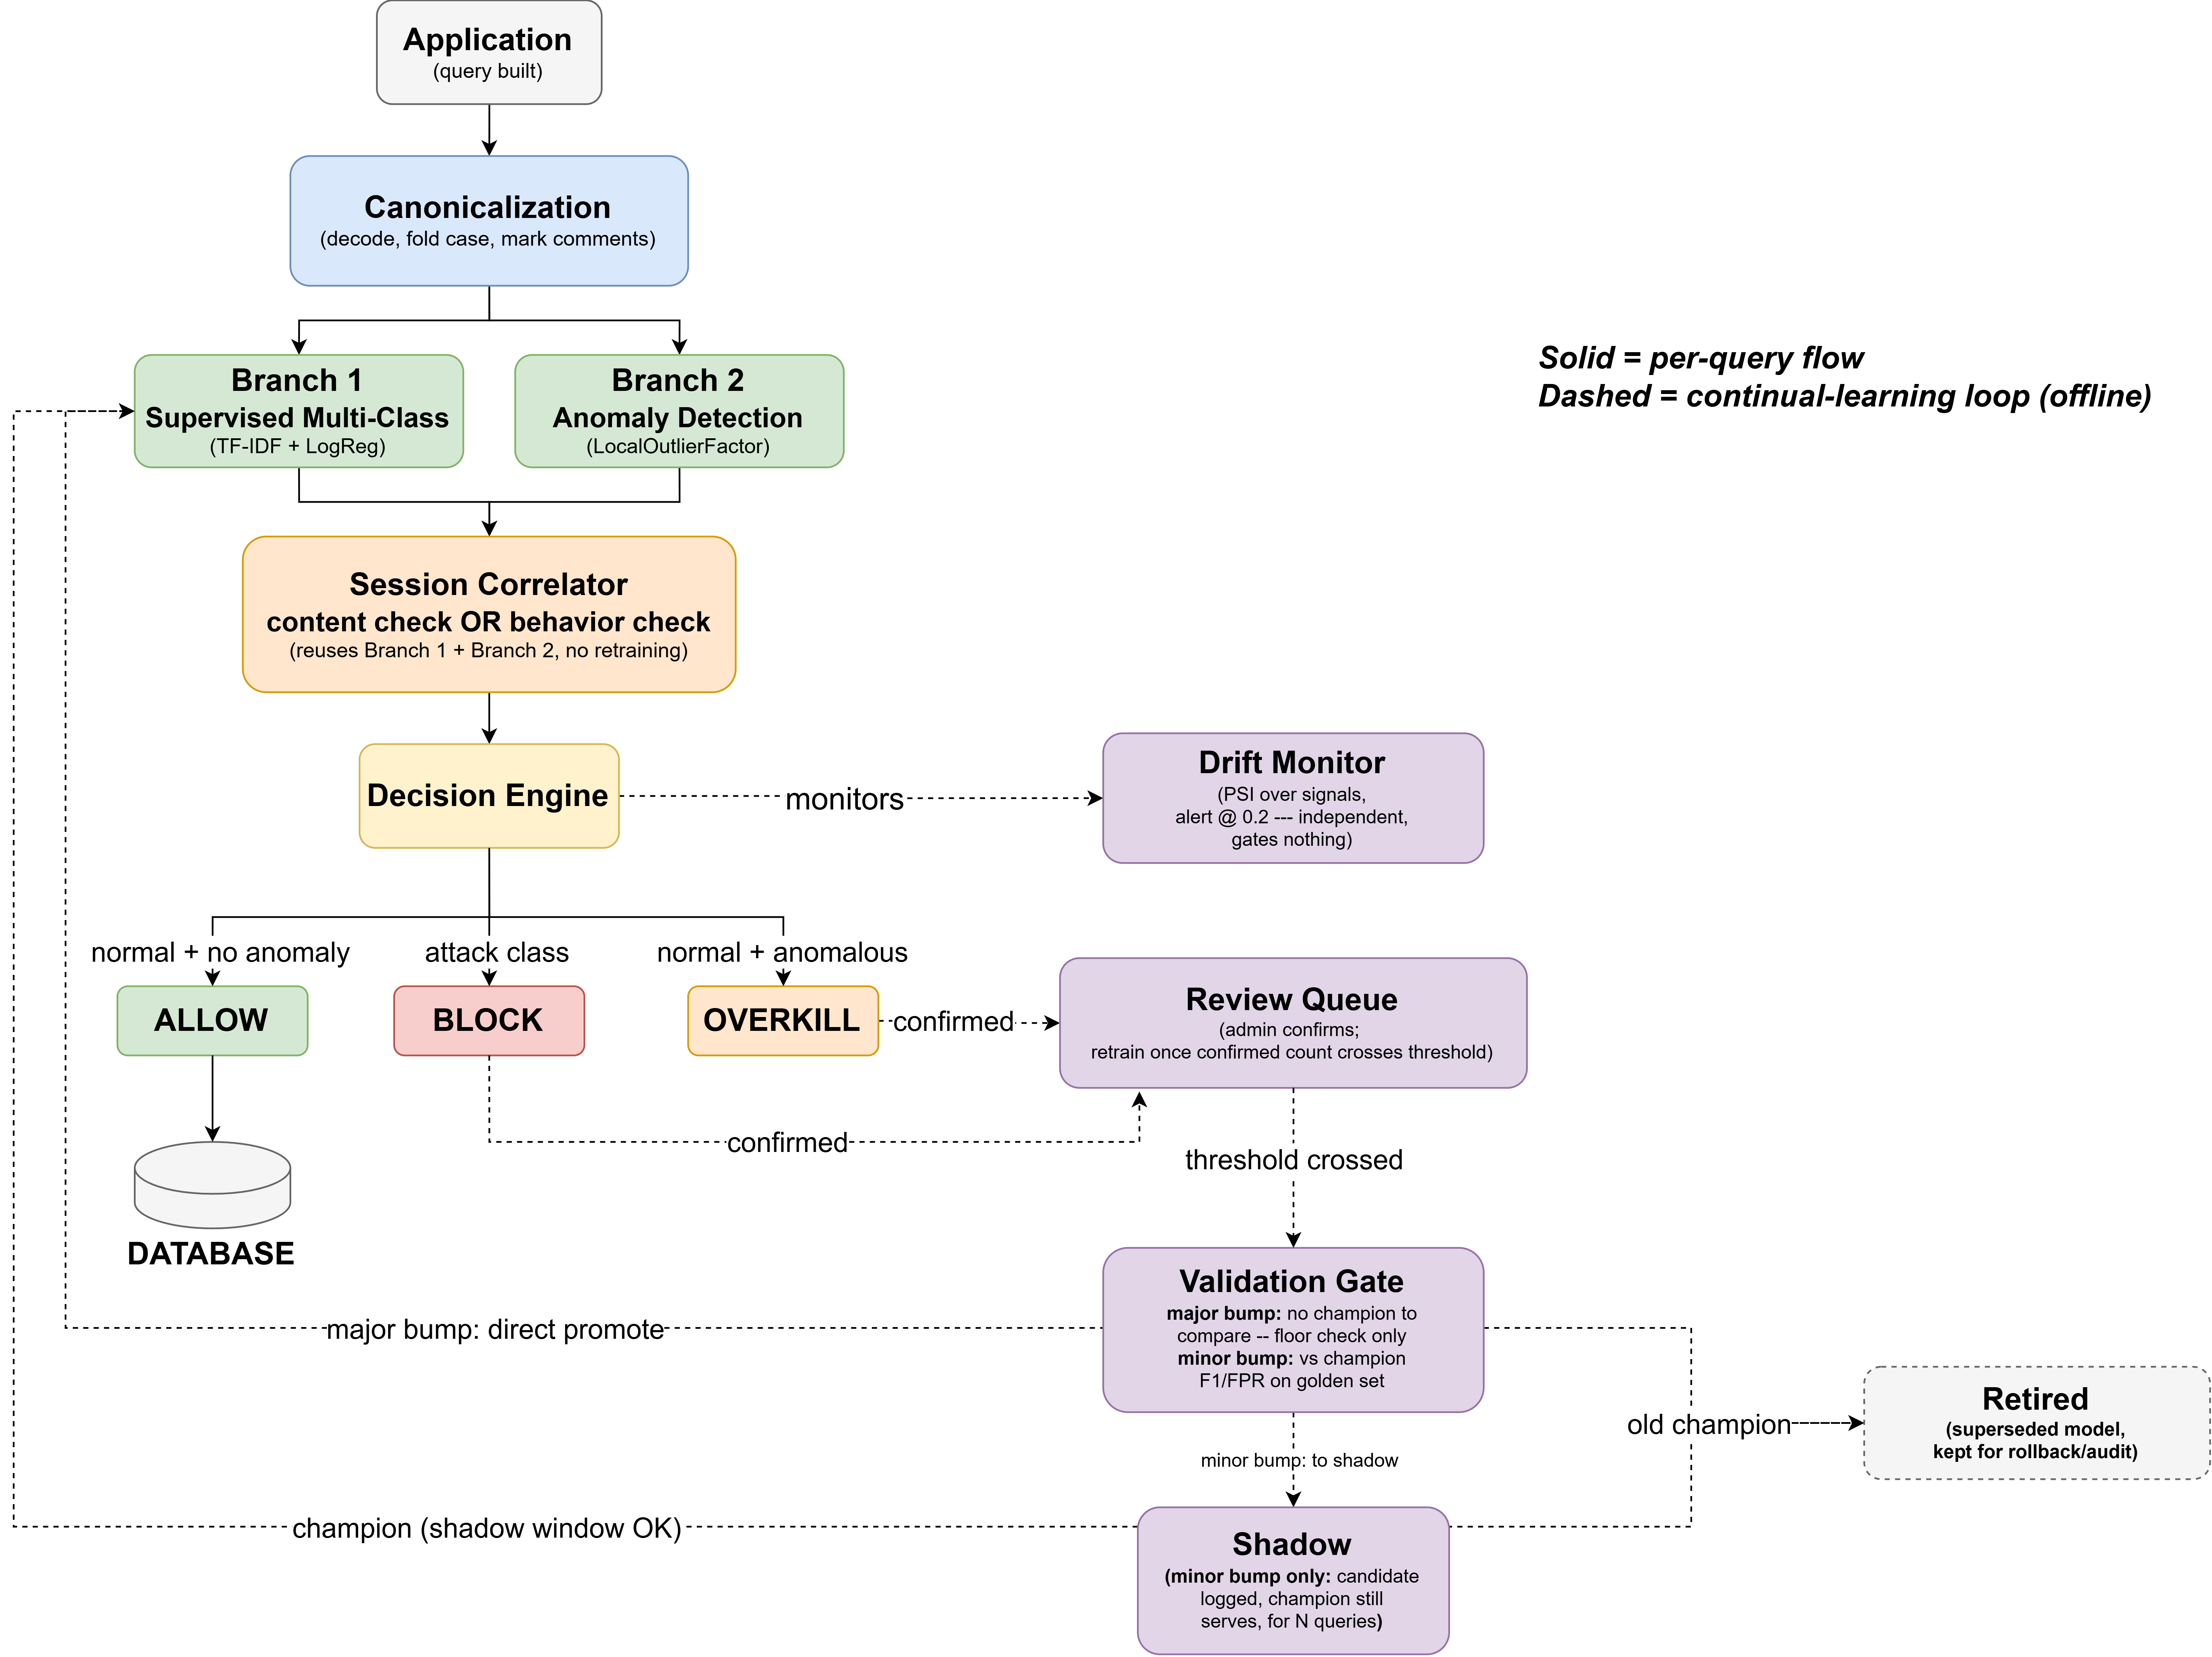
\includegraphics[width=0.9\textwidth]{architecturev2.0.drawio.png}}
\caption{Multi-branch detector at the database proxy.}
\label{fig:arch}
\end{figure*}

\begin{algorithm}[htbp]
\footnotesize
\caption{Multi-branch detection at Position B (per query)}
\label{alg:detect}
\begin{algorithmic}[1]
\REQUIRE query $q$, models $B_1,B_2$, correlator $S$
\STATE $q_c \leftarrow \text{canonicalize}(q)$
\STATE $(p, y_1) \leftarrow B_1.\text{predict}(q_c)$ \COMMENT{$p = 1 - P(\text{normal})$}
\STATE $s \leftarrow B_2.\text{score}(q_c)$
\STATE $is\_sqli \leftarrow (p \geq 0.5)$; $is\_anom \leftarrow (s > \tau_q)$
\STATE \textbf{if} $S.\text{is\_ready}$ \textbf{and} $S.\text{score\_session}([q])$ \textbf{then} \textbf{return} BLOCK
\STATE \textbf{if} $is\_sqli$ \textbf{then} \textbf{return} BLOCK
\STATE \textbf{if} $\neg is\_sqli \land is\_anom$ \textbf{then} \textbf{return} OVERKILL
\STATE \textbf{return} ALLOW
\end{algorithmic}
\end{algorithm}

\subsection{Canonicalization}
To reduce syntactic evasion, each statement is normalized before feature extraction: common encodings (URL, hex, \texttt{CHAR()}/\texttt{ASCII()}) are decoded, SQL keyword casing is normalized, and comment sequences (\texttt{/* */}, \texttt{--}) are \emph{marked as a feature} rather than deleted. The goal is to collapse equivalent syntactic variants so that trivial obfuscation does not change the model's input.

\subsection{Branch 1 - Supervised Multi-Class Classification}
Branch~1 assigns each query to one of five classes: \texttt{normal}, \texttt{union\_based}, \texttt{error\_based}, \texttt{boolean\_blind}, and \texttt{time\_blind}. We compare four candidate architectures (Section~\ref{sec:results}) and select TF-IDF features with a Logistic Regression classifier for its accuracy/latency/size trade-off. Multi-class (rather than binary) output lets the decision engine and human administrators reason about \emph{which} attack technique is detected.

\subsection{Branch 2 - Query-Level Anomaly Detection}
Branch~2 is trained on benign traffic only, learning the ``normal region'' of query behavior and emitting a continuous anomaly score for each query. Twelve lightweight features are used: four whole-string statistics (query length, special-character ratio, SQL-keyword count, Shannon entropy), a quote-imbalance count, and six ``local-peak'' features (longest same-type token run, maximum token length, token count, longest special-character run, longest digit run, and parenthesis imbalance) that measure a local run or token rather than a whole-string ratio, so that long parameter strings from HTTP-derived sources do not dilute the signal. A single global One-Class SVM decision boundary initially misclassified genuinely benign traffic from one data source as anomalous simply for not resembling another source's benign traffic; a per-source ensemble (one model per data source, OR'd) was tried next and rejected for an unacceptably high false-positive rate ($\approx$41\%). LocalOutlierFactor was adopted instead: its local-density notion judges each query against its own neighborhood rather than a single global boundary, which better accommodates a benign pool spanning structurally distinct sources. Training without any attack labels makes the branch, in principle, sensitive to attack shapes never seen by Branch~1-the property we probe in the zero-day study. The score also serves as an input feature to the Session Correlator.

\subsection{Session Correlator (Branch 3) - Session-Level Correlation}
The Session Correlator targets two attack patterns whose signal no query-level branch can see, because each step looks individually unremarkable: (1) blind SQLi (boolean-blind and time-blind), where an attacker recovers data one bit at a time via a bisection search spread across many queries in a session, and (2) query-splitting, where a single malicious statement is fragmented across multiple consecutive requests. Our first design is a sequence model (a Gated Recurrent Unit (GRU)) consuming, per step, Branch~1's classifier \emph{output} concatenated with Branch~2's anomaly score. A diagnostic investigation, focused on the blind-SQLi scenario, finds this premise does not hold: two consecutive Boolean-blind bisection steps differing only in their comparison bound have TF-IDF cosine similarity 0.961 at the vectorizer stage but near-identical probabilities after Branch~1's classifier (a lossy projection trained to separate attack \emph{type}, not to preserve content) - the very signal a session-level model needs is collapsed before it ever reaches the sequence model. Independently, the live decision engine already blocks most real Boolean/time-blind sessions per-query before enough steps accumulate for a sequence model to matter, and no principled fixed session length exists (real sessions range from a few to over a thousand steps). Section~\ref{sec:setup} describes how each of the two scenarios' session data is constructed, since only the blind-SQLi scenario's bisection structure is what exposed this failure. We therefore replaced the GRU with the Session Correlator: not a trained model, but two independent checks over an already-trained Branch~1 and Branch~2, OR'd together. The \emph{content check} concatenates a session's raw query text and re-scores it with Branch~1's existing classifier against a threshold calibrated separately for session-length text. The \emph{behavior check} aggregates Branch~2's per-query anomaly scores (mean, fraction above a calibrated threshold) across the session, run exactly as trained, per query, so no train/inference distribution shift is introduced. Both checks are calibrated on a disjoint TRAIN split and evaluated on a held-out TEST split (Section~\ref{sec:results}); each covers cases the other misses (content check: structurally-ordinary but lexically attack-like queries; behavior check: lexically-ambiguous but structurally anomalous ones), by design leaving one residual gap: an attacker evading both checks simultaneously, which no combination of the two existing branches' signals can close. Because the boolean-blind/time-blind session generator bisects toward a fixed target value (Section~\ref{sec:setup}), its output is deterministic per target; the target pool is therefore partitioned into disjoint train and test subsets \emph{before} session generation, so that no target used to calibrate the checks is ever reused at test time, and the held-out evaluation measures generalization to unseen targets rather than recall of seen ones.

\vspace{4pt}
Let $S=[q_1, \dots, q_n]$ be a session consisting of $n$ chronologically ordered queries from the same client. Denote\\[2pt]
\mbox{$p(S)=1-P_{B_1}(\text{normal}\mid \Vert_{i} q_i)$} for the concatenated text and \mbox{$s_i=B_2.\text{score}(q_i)$} per query. With calibrated thresholds $\tau_c,\tau_q,\tau_{mean},\tau_{frac}$, the checks are defined as:
\begingroup\small
\begin{equation}
\begin{aligned}
fires_c(S)&=\mathbb{I}[p(S)\geq \tau_c],\\
frac(S)&=\frac{1}{n}\sum_{i=1}^{n}\mathbb{I}[s_i>\tau_q],\\
fires_b(S)&=\mathbb{I}[\mu(S)\geq \tau_{mean}] \lor \mathbb{I}[frac(S)\geq \tau_{frac}]
\end{aligned}
\end{equation}
\endgroup
where $\mu(S)=(1/n)\sum s_i$ and the session verdict is\\[4pt]
\mbox{$fires_c(S) \lor fires_b(S)$}. Implemented operationally as in Algorithm~\ref{alg:correlator}.

\begin{algorithm}[htbp]
\footnotesize
\caption{SessionCorrelator: calibration and scoring (no gradient training)}
\label{alg:correlator}
\begin{algorithmic}[1]
\STATE \textbf{Calibration (on TRAIN sessions only):}
\STATE $\tau_q \leftarrow$ 90th percentile of
\STATE \hspace*{1em}$\{B_2.\text{score}(q) \mid q \in \text{benign TRAIN}\}$
\STATE $\tau_c \leftarrow \arg\max_{\tau} (\text{TPR}-\text{FPR})$ on
\STATE \hspace*{1em}$\{\text{concat}(S_{\text{train}}) \text{ scored by } B_1\}$
\STATE $\tau_{mean}, \tau_{frac} \leftarrow$ sweep mean and fraction-above-$\tau_q$
\STATE \hspace*{1em}on TRAIN
\STATE \textbf{Scoring a session $S=[q_1..q_n]$:}
\STATE $a_c \leftarrow 1-P_{B_1}(\text{normal} \mid \text{concat}(q_1..q_n))$; $fires_c \leftarrow (a_c \geq \tau_c)$
\STATE $scores \leftarrow [B_2.\text{score}(q_i) \; \forall i]$; $\mu \leftarrow \text{mean}(scores)$; $frac \leftarrow |\{s>\tau_q\}|/n$
\STATE $fires_b \leftarrow (\mu \geq \tau_{mean}) \lor (frac \geq \tau_{frac})$
\STATE \textbf{return} $fires_c \lor fires_b$ \COMMENT{content check OR behavior check}
\end{algorithmic}
\end{algorithm}

\subsection{Decision Engine and Overkill Policy}
A central decision engine combines the branch outputs into one verdict (Table~\ref{tab:decision}). Any query classified by Branch~1 as an attack class is \textsc{block}ed. A query classified \texttt{normal} but flagged anomalous by Branch~2 is held as an \emph{Overkill} case: it is not executed and is queued for administrator confirmation, defaulting to \emph{deny} on timeout. Confirmed decisions feed a continual-learning loop (proposed). This policy trades a small amount of friction on rare suspicious-but-benign queries for defense-in-depth against zero-days.

\begin{table}[htbp]
\caption{Decision policy combining the two query-level branches.}
\label{tab:decision}
\begin{center}
\begin{tabular}{@{}lll@{}}
\toprule
\textbf{Branch 1} & \textbf{Branch 2} & \textbf{Action} \\
\midrule
attack class & any & \textsc{block} + log \\
\texttt{normal} & anomalous & \textsc{overkill} (hold, deny on timeout) \\
\texttt{normal} & normal & \textsc{allow} \\
\bottomrule
\end{tabular}
\end{center}
\end{table}

\subsection{Continual-Learning Design}
Confirmed Overkill/Block decisions accumulate into a labeled pool that a continual-learning loop is designed to consume, so that the deployed model can improve without full retraining from scratch. Two parts run in parallel. \emph{Drift monitoring} continuously tracks the Population Stability Index (PSI) of five feature and confidence signals against a fixed reference window, alerting at PSI~$\geq$~0.2; it does not gate anything and can fire independently of the mechanism below. On the other path, a \emph{review queue} holds low-confidence and anomalous queries for administrator confirmation, and a volume-threshold policy decides when retraining actually happens: once confirmed samples relevant to a pending retrain cross a fixed count, a retrain job triggers automatically rather than on a fixed schedule. A \emph{validation gate} then decides whether the resulting candidate may replace the deployed model, distinguishing a \emph{major} bump (the label space itself changes, e.g.\ a genuinely new attack category) from a \emph{minor} one (same labels, more confirmed volume): a major bump has no prior model to compare against on equal footing, so the candidate is instead checked against an absolute floor - no regression on already-known classes, a minimum recall on the new one - and promoted directly if it clears that floor; a minor bump is compared against the current champion's F1/FPR on the frozen benchmark and must match or exceed it. Only a promoted minor-bump candidate then enters \emph{shadow}: its predictions are logged against a further window of traffic while the incumbent continues to serve decisions, and it becomes champion only if its shadow-observed FPR and F1 stay within tolerance of the gate-measured values, otherwise the incumbent is kept. A major-bump candidate skips shadow: there is no incumbent serving that class for it to be compared against, and the floor check above already carries the weight shadow exists to provide. Algorithm~\ref{alg:cl} summarizes the continual-learning loop. Every promotion retires the model it replaces - Shadow~$\rightarrow$~Champion~$\rightarrow$~Retired is the full lifecycle, with a retired model kept, not deleted, for rollback and audit. Section~\ref{sec:results} evaluates this loop as a full offline experiment.


\begin{algorithm}[htbp]
\footnotesize
\caption{Continual-learning loop (offline, Branch 1)}
\label{alg:cl}
\begin{algorithmic}[1]
\WHILE{streaming}
\STATE monitor PSI on 5 signals vs. reference; alert if $\text{PSI} \geq 0.2$
\STATE \hspace*{1em}for 2 sustained windows \COMMENT{drift, does not gate}
\STATE enqueue low-confidence and anomalous queries for admin review
\IF{$|\text{confirmed}| \geq 500$}
\STATE assemble $D' \leftarrow D_{\text{train}} \cup \text{confirmed}$
\STATE \hspace*{1em}(dedup by \texttt{query\_canonical})
\STATE seal data version $v=\text{infer\_bump}(v_{\text{old}}, v_{\text{new}})$
\IF{$v$ is major}
\STATE check floor: no known-class recall drop $>0.02$
\STATE \hspace*{1em}and new-class recall $\geq 0.80$; promote directly if pass
\ELSE
\STATE gate: $F1_{cand} \geq F1_{champ} \land \text{FPR}_{cand} \leq \text{FPR}_{champ}$
\STATE \hspace*{1em}\COMMENT{shadow 2000 queries if pass}
\ENDIF
\ENDIF
\ENDWHILE
\end{algorithmic}
\end{algorithm}

\section{Dataset and Experimental Setup}\label{sec:setup}

\subsection{Data Sources}
Four public datasets are combined: \emph{SQLiV3} (D1, a Kaggle SQLi query collection; license provenance unclear, see Section~\ref{sec:discussion}); \emph{CSIC 2010} (D2, HTTP traffic, used both for benign enrichment and, held out, as a labeled anomalous evaluation set); \emph{payload-box} (D3, MIT-licensed SQLi payload strings); and \emph{SR-BH 2020} (D4, a CC0 honeypot dataset of 527{,}813 rows, 250{,}285 originally tagged \texttt{SQL Injection}). Because D4's labels are coarse and multi-attack (Common Attack Pattern Enumeration and Classification (CAPEC)-tagged), rows were re-tagged into SQLi sub-types by rule-based matching rather than trusted as-is.

\subsection{Branch 1 Dataset}
Sub-type re-labeling of D4 supplies most per-class volume. The \texttt{stacked} class has \emph{zero} naturally-occurring samples across D1/D3/D4; 363 synthetic samples are templated to represent it, but all four candidate models achieved 100\% recall on them-evidence of trivial separability rather than a solved sub-problem-so \texttt{stacked} is excluded from the reported training set entirely (the continual-learning experiment in Section~\ref{sec:results} instead holds out a real class, \texttt{union\_based}, from its own separate training pool - see Section~\ref{sec:results} for why). Content-based signature filtering (independent of source labels) removed mislabeled attacks from the \texttt{normal} pool over three iterative rounds. Before splitting, \texttt{query\_canonical} text is deduplicated, so no query text appears verbatim in both the train and test partitions; this also lets class balancing draw from a larger pool of distinct rows. The final dataset used for training is 67{,}796 rows over five classes, split 54{,}236 training and 13{,}560 test (stratified, seed~$=42$); the three largest classes were undersampled to $\approx$15{,}000 rows each. F1-macro is the headline metric because accuracy would be distorted by the underlying class imbalance.

\subsection{Branch 2 Dataset}
Branch~2 pools clean benign rows from D1, D2, and D4, using a broader content filter that rejects \emph{any} attack-like traffic (not only SQLi). D2 and D4 are captured as full HTTP requests (scheme, host, path, query/body), not raw SQL; since the system consumes only the query/parameter text an application would build (Section~\ref{sec:system}), each such row is first stripped to its query-string/body parameters, and rows with nothing left after stripping (bare static-asset requests) are dropped. After filtering, de-duplication, and stripping, the benign pool contains 36{,}502 rows (28{,}573 training and 7{,}929 test). A held-out evaluation set of 270{,}002 confirmed-SQLi rows spanning D1, D2, and D4 (D4 via its own CAPEC ``SQL Injection'' column) is used only for evaluation, not training.

\subsection{Session Correlator Dataset}
No public dataset provides session-level SQLi labels, so sessions for the two target scenarios (Section~\ref{sec:system}) are constructed differently, reflecting how each attack actually unfolds. Blind-SQLi sessions (boolean-blind, time-blind) run the same bisection algorithm real SQLi tools use - length probing followed by per-character ASCII probing, $\sim$7 requests per character - against a real, self-hosted SQLite database, so every probe's true/false outcome is a genuine row-count difference or a genuine measured \texttt{SLEEP()} delay, not a templated guess; this is the scenario whose bisection structure exposed the GRU's failure (Section~\ref{sec:system}). Query-splitting sessions instead use heuristic token-fragmentation of a single real attack payload across consecutive requests, since no bisection-style shared search exists for this attack type. Together this yields 1{,}400 sessions across four classes (benign, boolean-blind, time-blind, query-splitting), split 1{,}120 training and 280 test. The 100-user synthetic target pool used for boolean-blind/time-blind generation is itself partitioned into disjoint train/test target subsets before sessions are generated (Section~\ref{sec:system}). Collecting an independent dataset from real \texttt{sqlmap} traffic against a deliberately vulnerable application is future work (Section~\ref{sec:conclusion}); Section~\ref{sec:discussion} states plainly what this means for how the Session Correlator results below should be read.

\subsection{Evaluation Protocol}
Metric choice follows from each branch's task rather than a single convention across all three. Branch~1 is a multi-class classifier over an imbalanced label set, so F1-macro (not accuracy, which the majority classes would inflate) is the headline metric, alongside per-class precision/recall/F1, a confusion matrix, and per-class ROC to show where errors concentrate. Branch~2 is a one-class anomaly detector with no fixed decision boundary a priori, so we report FPR and detection rate at a specific operating point (the deployment-relevant trade-off), AUC (a threshold-independent summary of ranking quality), and a 21-point threshold sweep to make the trade-off curve, not just one point on it, inspectable. The Session Correlator issues a binary per-class flag from two independently OR'd checks, so FPR on benign sessions and detection rate per attack class are reported separately for each check alone and combined - an ablation, not just a combined number, so neither check's contribution is left unmeasured. All experiments are deterministic (seed~$=42$); latency was measured on a single RTX~3050 (6~GB) workstation.

\section{Experimental Results}\label{sec:results}

\subsection{Branch 1 - Supervised Multi-Class}
Table~\ref{tab:b1arch} compares the four candidate architectures. LightGBM reaches the highest F1-macro (0.998) but at $\approx$115$\times$ the per-query latency (60.4~ms, unworkable for a real-time proxy); DistilBERT (0.996) needs a GPU, a 256~MB artifact, and $\approx$25~minutes to train, for no deployment benefit. The CNN tokenizer (0.991) is essentially tied with the chosen Logistic Regression (0.991) while being faster and an order of magnitude smaller, but is kept as a fallback rather than the primary model since it still requires a custom tokenizer and a deep-learning framework dependency that Logistic Regression does not. TF-IDF~+~Logistic Regression was selected for its negligible F1 cost relative to the two higher-scoring models, and the simplicity of a pure linear model with no extra deep-learning framework dependency.

\begin{table}[t]
\caption{Branch~1 architecture comparison (5-class data, post-deduplication).}
\label{tab:b1arch}
\begin{center}
\begin{tabular}{@{}lcccc@{}}
\toprule
\textbf{Model} & \textbf{F1-macro} & \textbf{p50 lat.} & \textbf{Size} & \textbf{Train} \\
\midrule
TF-IDF + LogReg (chosen) & 0.991 & 0.5~ms & 3.7~MB & 13~s \\
TF-IDF + LightGBM & 0.998 & 60.4~ms & 5.9~MB & 195~s \\
DistilBERT & 0.996 & 2.8~ms$^{\ast}$ & 256~MB & 1{,}499~s \\
CNN + SQL-tokenizer & 0.991 & 0.3~ms & 118~KB & 10~s \\
\bottomrule
\multicolumn{5}{l}{\footnotesize DR = detection rate; FPR = false-positive rate.}\\
\end{tabular}
\end{center}
\end{table}

After excluding \texttt{stacked}, deduplicating query text before the train/test split, and retraining on the five real classes, the chosen model reaches F1-macro~=~0.9907. Table~\ref{tab:b1perclass} gives the per-class breakdown; the only material confusion is between \texttt{normal} and \texttt{boolean\_blind}, consistent with the $\approx$13\% label noise measured in the \texttt{boolean\_blind} catch-all class (Section~\ref{sec:discussion}). \texttt{time\_blind} reaches an exact 1.000 on all three metrics - checked directly rather than accepted at face value, given this project's own history of misleadingly-perfect scores: every one of its 15{,}000 rows contains one of a small, deterministic keyword family (\texttt{SLEEP(}, \texttt{BENCHMARK(}, \texttt{WAITFOR DELAY}, \texttt{PG\_SLEEP(}) that the labeling rule itself requires, and which never occurs in any other class's rows; the 15{,}000 texts are also all distinct, ruling out duplicate memorization. Perfect separation here reflects a near-unique lexical signature the tagging rule guarantees, not overfitting - though it also means this number does not test generalization to time-based techniques that avoid this specific keyword family. Per-class ROC curves are shown in Fig.~\ref{fig:b1roc}. This F1 is measured on a clean test split, not on adversarially perturbed input, and should be read accordingly.

\begin{table}[t]
\caption{Branch~1 per-class results (test set, $n=13{,}560$).}
\label{tab:b1perclass}
\begin{center}
\begin{tabular}{@{}lcccc@{}}
\toprule
\textbf{Class} & \textbf{Prec.} & \textbf{Recall} & \textbf{F1} & \textbf{Support} \\
\midrule
\texttt{normal}        & 0.986 & 0.968 & 0.977 & 3{,}000 \\
\texttt{union\_based}  & 0.999 & 0.994 & 0.996 & 3{,}000 \\
\texttt{error\_based}  & 0.999 & 1.000 & 0.999 & 1{,}560 \\
\texttt{boolean\_blind}& 0.969 & 0.992 & 0.981 & 3{,}000 \\
\texttt{time\_blind}   & 1.000 & 1.000 & 1.000 & 3{,}000 \\
\bottomrule
\multicolumn{5}{l}{\footnotesize DR = detection rate; FPR = false-positive rate.}
\end{tabular}
\end{center}
\end{table}

\begin{figure}[htbp]
\centerline{
\includegraphics[width=\columnwidth]{branch1_roc_per_class.png}}
\caption{Branch~1 per-class ROC curves.}
\label{fig:b1roc}
\end{figure}

\subsection{Branch 2 - Query-Level Anomaly Detection}
Table~\ref{tab:b2} compares three anomaly algorithms on the same benign/anomalous pools (Section~\ref{sec:setup}). One-Class SVM under-performs on this 12-feature representation; Isolation Forest is a substantial improvement but still leaves most attacks undetected at its operating point; LocalOutlierFactor was selected for its higher AUC and detection rate. At its chosen operating point (contamination~=~0.05), it produces 427 false positives on 7{,}929 benign queries (FPR~=~5.4\%) and flags 81.4\% of the 270{,}002 held-out anomalous queries, with average precision~=~0.996. Fig.~\ref{fig:b2} shows the resulting 21-point threshold sweep: the false-positive rate falls sharply over the first few thresholds, while the detection rate declines more gradually across the same range, so the steep initial region trades a small detection loss for a large FPR reduction. Past roughly the tenth threshold, further FPR reduction flattens while detection keeps falling, making that region unattractive; the chosen operating point (contamination~=~0.05) sits inside the steep initial region, where the FPR/detection trade-off is most favorable.

\begin{table}[htbp]
\caption{Branch~2 algorithm comparison (same benign/anomalous pools).}
\label{tab:b2}
\begin{center}
\begin{tabular}{@{}lcccc@{}}
\toprule
\textbf{Algorithm} & \textbf{Contam.} & \textbf{FPR} & \textbf{Detection} & \textbf{AUC} \\
\midrule
One-Class SVM & 0.001 & 0.23\% & 7.83\% & 0.422 \\
Isolation Forest & 0.01 & 1.90\% & 37.60\% & 0.860 \\
LocalOutlierFactor (chosen) & 0.05 & 5.39\% & 81.37\% & 0.929 \\
\bottomrule
\multicolumn{5}{l}{\footnotesize DR = detection rate; FPR = false-positive rate.}
\end{tabular}
\end{center}
\end{table}
\vspace{-6pt}
\begin{figure}[htbp]
\centerline{
\includegraphics[width=0.9\columnwidth]{branch2_threshold_tradeoff.png}}
\caption{Branch~2 threshold trade-off: false-positive rate vs.\ detection rate across 21 operating points.}
\label{fig:b2}
\end{figure}

\FloatBarrier
\subsection{Zero-Day Generalization Study}
To probe robustness to \emph{unseen} attack categories, we run a leave-one-out protocol: for each SQLi class, that class is removed and Branch~1 is retrained on the remaining four; Branch~2 is not retrained per fold, since it is trained only on benign traffic and never sees attack labels to begin with, so the same fixed anomaly detector is evaluated against every held-out class's queries. We report the Branch~1 \emph{miss rate} (fraction predicted \texttt{normal}, i.e.\ bypassing the supervised branch), the Branch~2 detection rate on the same held-out queries, and their \emph{combined coverage} (fraction caught by at least one branch) in Table~\ref{tab:zeroday}.

\begin{table}[t]
\caption{Leave-one-out zero-day results. B1 miss = fraction of the unseen class predicted \texttt{normal} (bypass); B2 detection = fraction independently flagged anomalous; Combined = fraction caught by either branch.}
\label{tab:zeroday}
\begin{center}
\begin{tabular}{@{}lccc@{}}
\toprule
\textbf{Unseen class} & \textbf{B1 miss} & \textbf{B2 detection} & \textbf{Combined} \\
\midrule
\texttt{union\_based}   & 2.6\%  & 99.1\% & 99.8\% \\
\texttt{error\_based}   & 0.0\%  & 98.3\% & 100.0\% \\
\texttt{boolean\_blind} & 86.5\% & 87.8\% & 88.8\% \\
\texttt{time\_blind}    & 0.1\%  & 99.0\% & 100.0\% \\
\bottomrule
\end{tabular}
\end{center}
\end{table}

Two findings stand out. First, supervised classification generalizes well to unseen classes that are \emph{structurally distinctive}: when \texttt{union\_based}, \texttt{error\_based}, or \texttt{time\_blind} is withheld, Branch~1 still flags almost all of its queries as \emph{some} attack (miss rate $\leq$2.6\%), because their tokens differ sharply from benign traffic - and, independently, the anomaly branch also catches nearly all of them (98.3--99.1\%), since these payloads' distinctive structure registers as anomalous regardless of whether Branch~1 was trained to recognize the specific class. Second, and critically, \texttt{boolean\_blind} is still the failure mode, but not as starkly as a single branch's numbers suggest: with that class unseen, Branch~1 misclassifies 86.5\% of its queries as \texttt{normal}, because Boolean-blind payloads are lexically close to legitimate queries - yet the anomaly branch independently catches 87.8\% of the same queries on structural grounds alone, and the two combined still leave 11.2\% uncaught, the lowest combined coverage of any class by a wide margin (88.8\% vs.\ $\geq$99.8\% elsewhere). This residual gap, not an absence of anomaly coverage, is the empirical motivation for session-level correlation: query-level detection alone still misses roughly one in nine unseen boolean-blind queries, and closing that gap is precisely what accumulating signal across a session is positioned to do. At the session level, this same zero-day condition closes entirely: the Session Correlator's behavior check, which depends only on Branch~2 and is therefore unaffected by Branch~1's blindness, independently flags all 70 held-out \texttt{boolean\_blind} sessions (Section~\ref{sec:results}) - though this is a session-level, not query-level, result on a different (self-generated) evaluation set, and should be read as complementary evidence rather than a directly comparable number.

\subsection{Session Correlator}
Table~\ref{tab:b3} reports the mandatory ablation on the 280-session held-out self-hosted test set (disjoint train/test target pools, Section~\ref{sec:system}): each row runs \emph{only} the named mechanism (the other disabled) to isolate its individual contribution, except the last, which is how the deployed system actually runs the two OR'd together. Content check (session text) and Combined (OR) reach zero observed false positives and perfect detection on all three attack classes; Behavior check (B2 scores), run alone, does not fully catch \texttt{query\_splitting} (0.457) - a genuine, distinct blind spot the content check closes, which is why the two are OR'd rather than either being used alone.

\begin{table}[t]
\caption{Session Correlator ablation ($n=280$).}
\label{tab:b3}
\begin{center}
\begin{tabular}{@{}lcccc@{}}
\toprule
\textbf{Configuration} & \textbf{FPR} & \textbf{DR bool.} & \textbf{DR time} & \textbf{DR split} \\
\midrule
Content check  & 0/70 & 1.0 & 1.0 & 1.0 \\
Behavior check & 0/70 & 1.0 & 1.0 & 0.457 \\
Combined (OR)  & 0/70 & 1.0 & 1.0 & 1.0 \\
\bottomrule
\end{tabular}
\end{center}
\end{table}

A separate zero-day ablation re-scores the content check on boolean-blind test sessions using the leave-one-out Branch~1 variant from Section~\ref{sec:results}'s zero-day study (never trained on boolean-blind). Detection rate drops to 0.0, with mean attack probability stuck around 0.22 regardless of how much of the session is concatenated - concatenation amplifies a signal Branch~1 already recognizes; it cannot rescue a classifier that never learned the class at all. We report this as a stated limitation, not as a caveat that quietly disappears: it is a direct consequence of the Session Correlator re-using Branch~1's signal rather than learning an independent one.

\emph{Reading these numbers narrowly.} Zero observed false positives on 70 benign sessions bounds the true FPR only loosely (a 95\% Wilson interval reaches roughly 4\%), and benign sessions are drawn from the same generation process Branch~1 and Branch~2 were built around, not independently-captured production traffic. The disjoint train/test target-pool design (Section~\ref{sec:system}) means these numbers at least reflect generalization to unseen targets within that generation process, which is a real, if narrow, form of held-out evaluation. We read this table as evidence the correlation mechanism works as designed - each check independently covers the weak-signal cases the other might miss, which we verified directly rather than assumed - and not yet as evidence of generalization to adversarially-diverse real traffic, which independently-captured attacker traffic (Section~\ref{sec:conclusion}) is intended to test.

\subsection{Continual Learning}
Unlike \texttt{stacked} in Branch~1's main results, this experiment holds out a \emph{real} class: \texttt{union\_based} is entirely absent from an initial training pool (M0, 20{,}194 rows over the remaining four classes - deliberately about half of what those four classes have available, so a later retrain has real held-back volume to draw on, not merely a few leftover rows), and a frozen golden set (6{,}780 rows, all five classes, disjoint from anything below) is set aside for evaluation throughout. A two-pour replay stream follows (12{,}955 queries, padded with real held-out benign traffic from Branch~2's pool): \emph{Scenario~1} interleaves \texttt{union\_based} into ordinary traffic after a quiet head; \emph{Scenario~2} is more volume of the four known classes only, no new class. A review queue and a drift monitor watch both pours independently.

Pre-bump: M0 facing a class it has never seen. On the golden set's four known classes, M0 reaches F1-macro~=~0.9868 (FPR~=~0.0333). On \texttt{union\_based}'s golden rows (n~=~1{,}500, unseen by M0), Branch~1 alone misses 12.3\% (predicts \texttt{normal}); Branch~2 - fixed for this entire experiment, exactly as in the zero-day study above, since it is benign-only and never sees attack labels - independently flags 99.5\% of them, for 99.7\% combined coverage. (This is not the same number as Table~\ref{tab:zeroday}'s 2.6\%/99.1\%/99.8\% for the same class: that study trains Branch~1 on one large 80/20 split, whereas M0 here trains on deliberately half of the four known classes' available volume, to keep ``half the data, missing one label'' a true description of this experiment's Base rather than an overstatement.)

The review queue triggers a major bump. As \texttt{union\_based} traffic streams in, flagged occurrences accumulate in the review queue; once 500 confirmed \texttt{union\_based} samples are reached - 47.5\% through Scenario~1's pour - a retrain triggers automatically. The resulting candidate (M1, 21{,}463 rows) reaches F1-macro~=~0.9806 on the full five-class golden set (FPR~=~0.0333) and 95.9\% recall on \texttt{union\_based}, clearing the promotion floor (no known-class regression, new-class recall~$\geq$~0.80); with no prior model to compare against on equal footing, M1 is promoted directly and M0 is retired. On the remainder of Scenario~1's pour - traffic M1 was never trained on - it independently recalls 95.4\% of the 1{,}486 remaining \texttt{union\_based} occurrences, confirming the golden-set number holds on genuinely fresh stream data.

Ablation: is the gain from the class, or just from more rows? A control retrains M0's pool with the identical +1{,}269-row budget, resampled entirely from the four known classes - no \texttt{union\_based} at all. Fig.~\ref{fig:cl-ablation} shows the result: 0.000 recall for the control versus 0.959 for M1, on identical row counts. Since row count is held fixed and only composition varies, the gain is attributable to learning the class itself, not to having more training data.

\begin{figure}[t]
\centerline{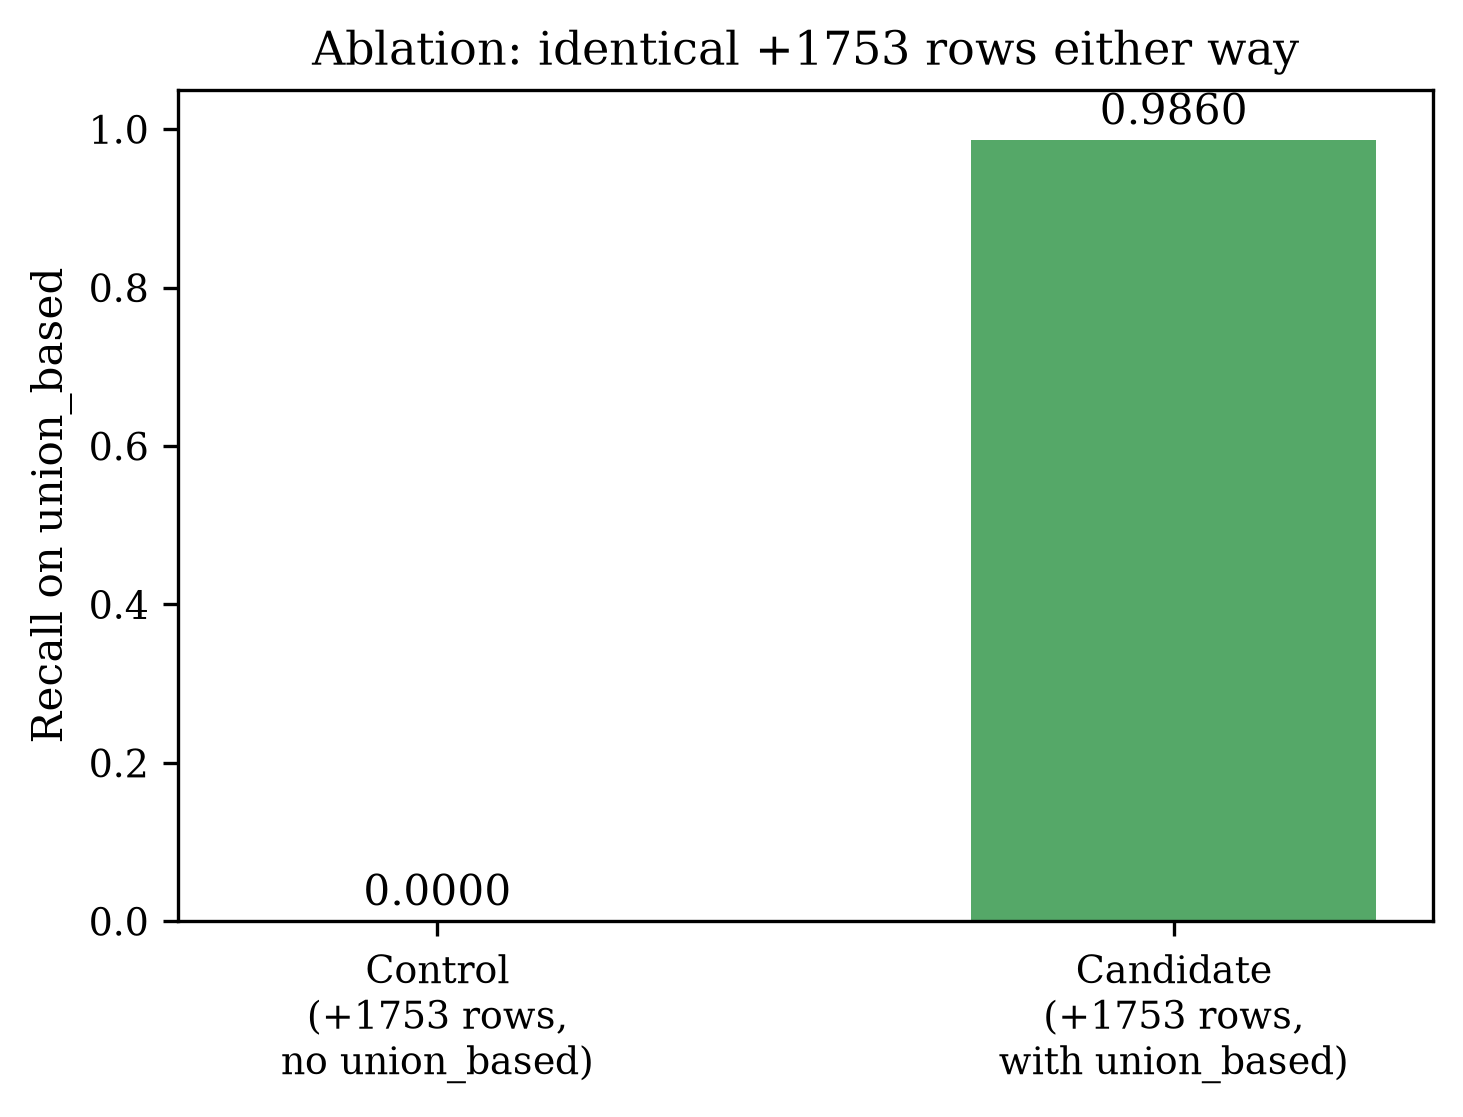
\includegraphics[width=\columnwidth]{cl_scenario_ablation.png}}
\caption{Ablation: recall on \texttt{union\_based} with (0.959) vs.\ without (0.000) the class present in an identical +1{,}269-row retrain sample.}
\label{fig:cl-ablation}
\end{figure}

Drift monitoring sees it too, at this concentration. Fig.~\ref{fig:cl-drift} (top) tracks five PSI signals through Scenario~1 against M0: the flagged-traffic structural-feature signal crosses the 0.2 alert threshold by window~2 and is confirmed (two sustained windows) by window~3 - the same window the queue's own retrain trigger falls in. This does not overturn a low-concentration negative result reported for a rare ($<$1\%) synthetic class elsewhere in this project's development; at the substantially higher concentration used here (\texttt{union\_based} $\approx$29\% of Scenario~1's traffic, sized to what the $\approx$8.7K-row benign-padding budget available at experiment scale could plausibly support, not to match a specific production rate), drift and the review queue agree rather than the queue being the only signal that notices.

Scenario 2: a minor bump, then shadow. With M1 now champion, Scenario~2 replays known-class volume only. Once 500 confirmed samples accumulate (position 2{,}093 of 6{,}026), a class-balanced pool (112 rows - the smallest confirmed class, \texttt{normal} false positives, sets the size) is added and M2 is trained. On the full golden set, M2 reaches F1-macro~=~0.9811 and FPR~=~0.0293, a 12\% relative FPR cut versus M1 with no per-class regression; the gate promotes it to \emph{shadow}. Observed against the next 2{,}000 queries (predictions logged, M1 still deciding live), M2's FPR (1.0\%) and F1-macro (0.9863) both stay within tolerance of the gate-measured values, so M2 is promoted to champion and M1 is retired.

\begin{figure}[t]
\centerline{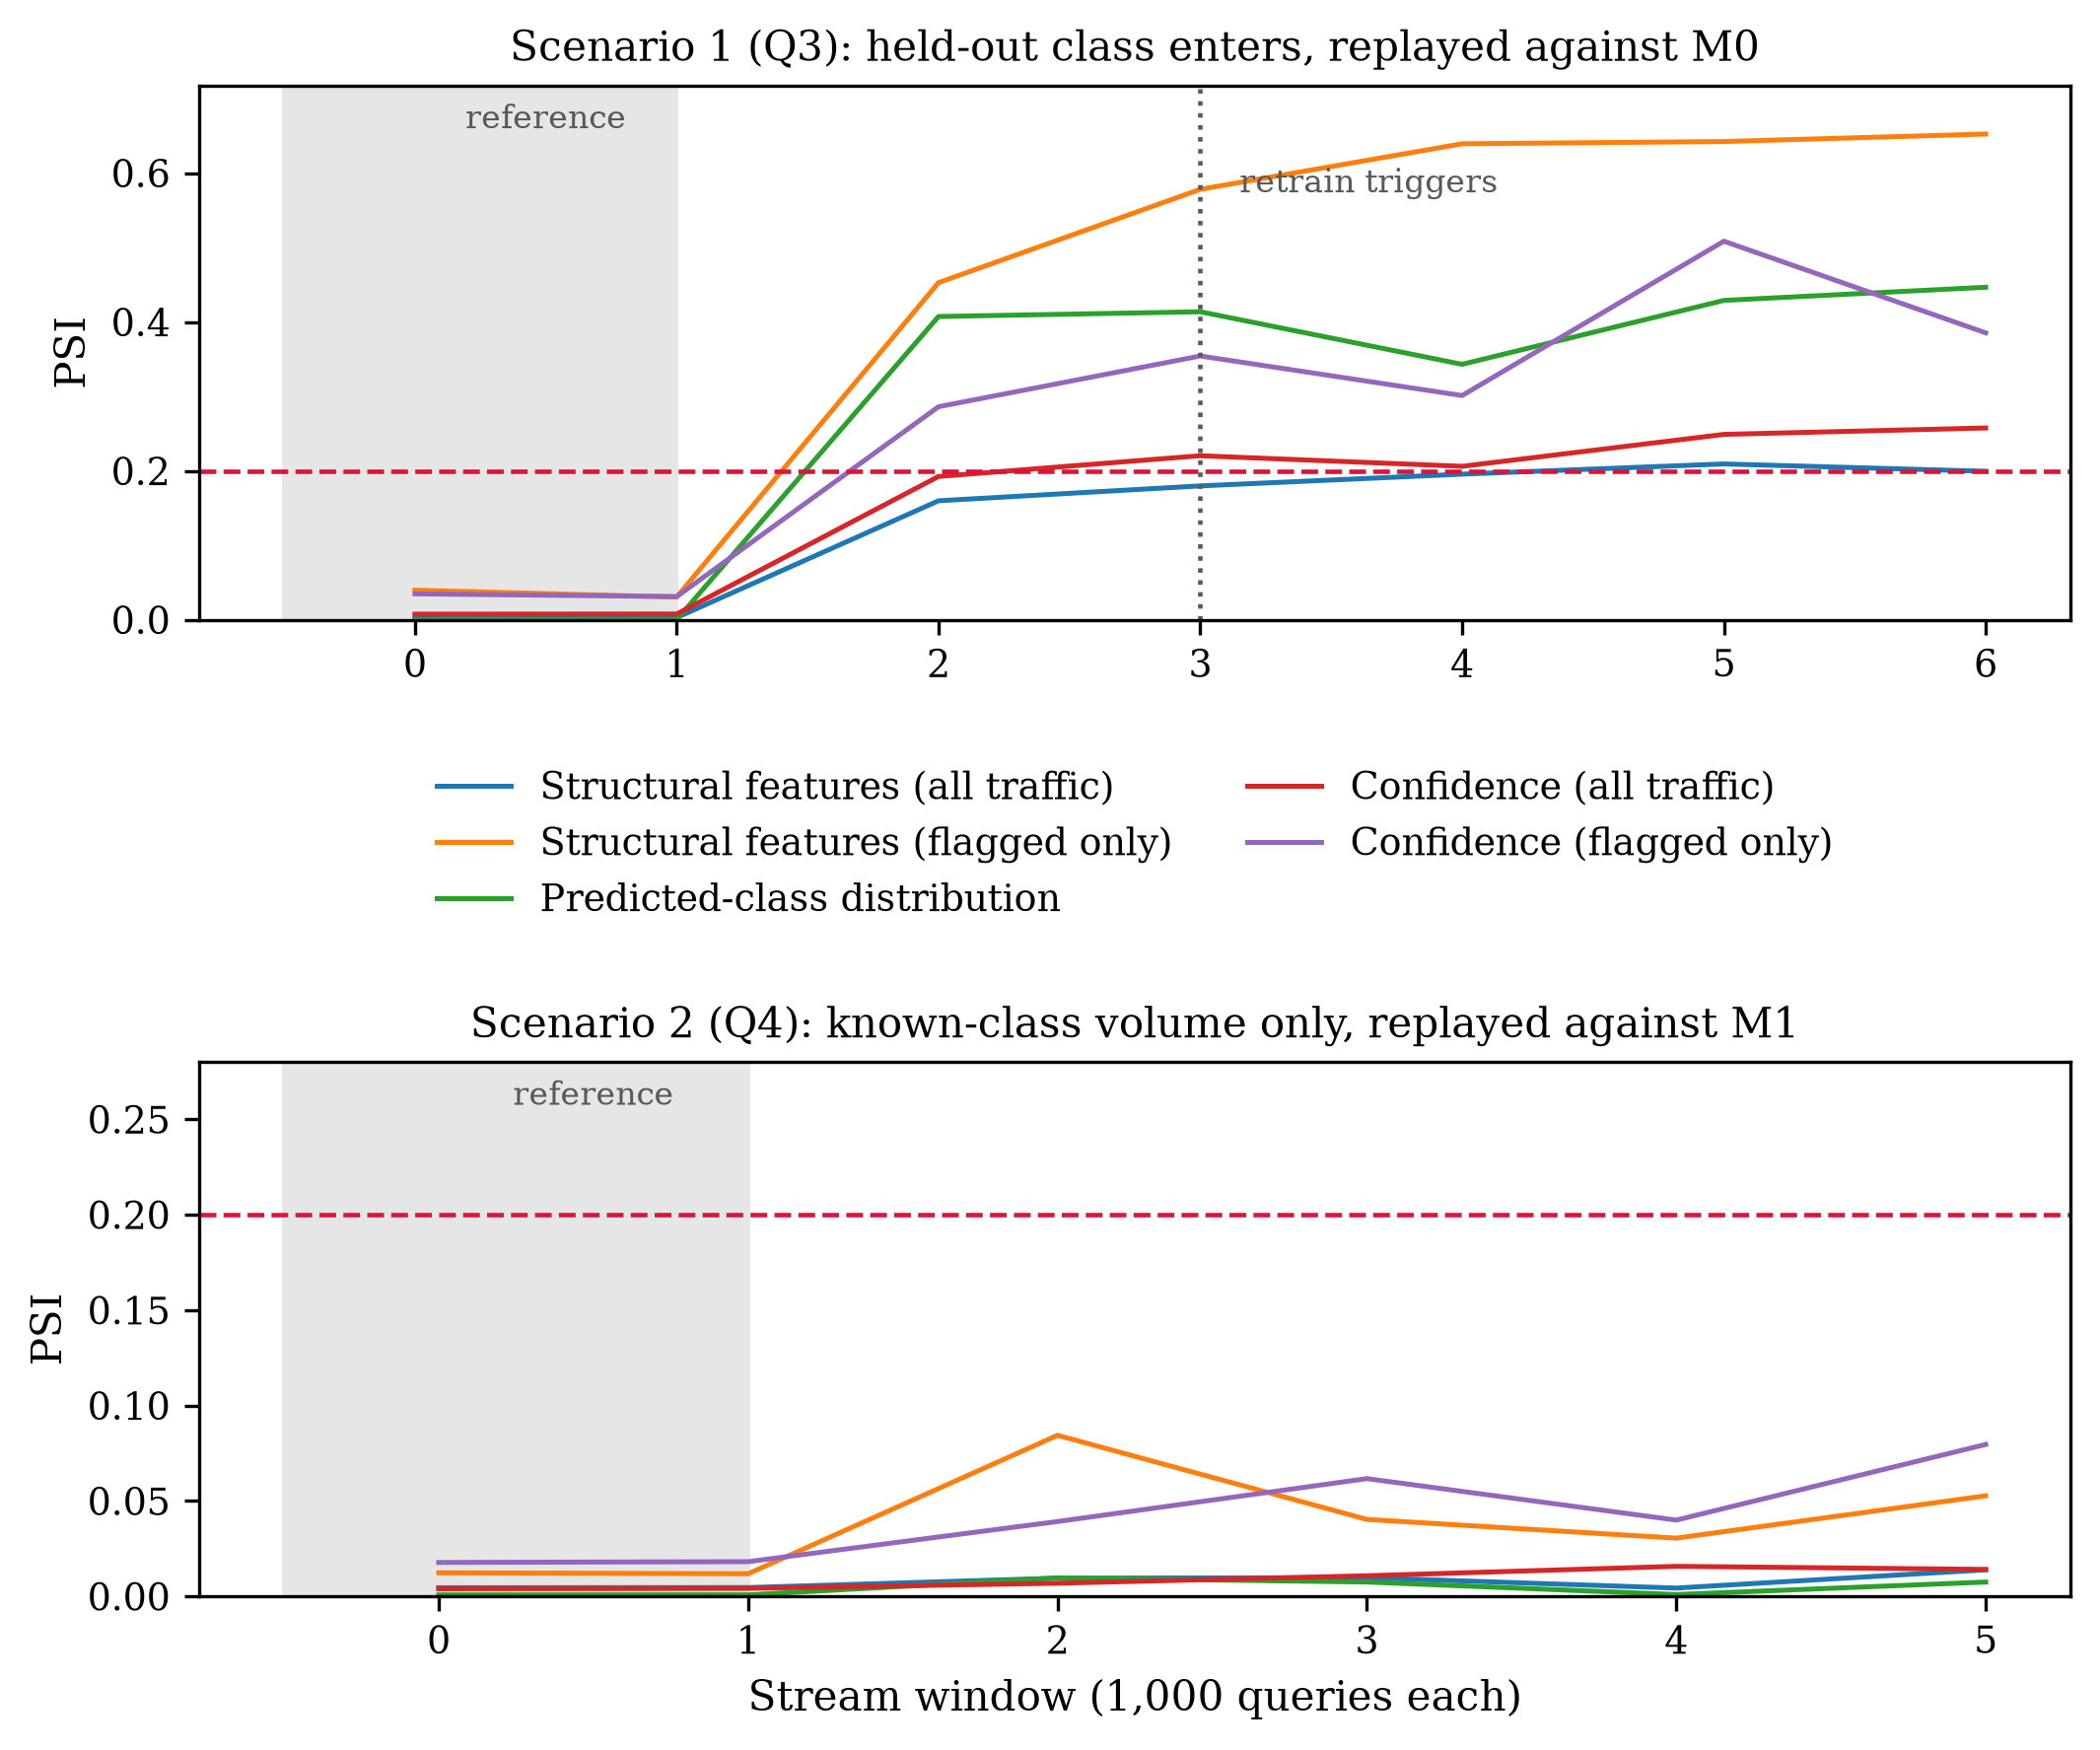
\includegraphics[width=\columnwidth]{cl_scenario_drift.png}}
\caption{PSI drift signals through Scenario~1 (vs.\ M0, top) and Scenario~2 (vs.\ M1, bottom). Scenario~1 crosses the alert threshold as \texttt{union\_based} enters; Scenario~2 stays flat throughout.}
\label{fig:cl-drift}
\end{figure}

Fig.~\ref{fig:cl-drift} (bottom) confirms the expected contrast: replayed against M1, Scenario~2's drift signals stay flat throughout - ordinary volume growth alone does not look like drift.

\emph{Reading these numbers narrowly.} Both pours are padded with real benign traffic, but at a higher attack concentration than production would see, bounded by the $\approx$8.7K held-out benign rows available for padding at this scale; \texttt{union\_based}'s pour is similarly a subsample (2{,}000 of the 13{,}500 non-golden rows available) sized for the same reason, not because more of the class was unavailable. Labelling is simulated (ground truth stands in for a human reviewer), and traffic is a replay of held-out data, not live production traffic. The review queue and validation gate are implemented and tested as a library, but production wiring into the deployed service (an administrator-facing queue, a live drift dashboard) is not yet complete for all branches - this offline result validates the mechanism, not a running deployment.

\subsection{Latency Budget}
End-to-end per-query latency is estimated from measured per-branch costs rather than benchmarked under load on the live service. Branch~1 inference is 0.5~ms (Table~\ref{tab:b1arch}). Branch~2's LocalOutlierFactor scores each query against its stored training set (a $k$-nearest-neighbor lookup, not a fixed decision boundary like the One-Class SVM baseline), which costs substantially more than a linear model: an offline benchmark on the same workstation measures $\approx$15--18~ms per query. Decision-engine logic is negligible. The combined query-level budget is therefore on the order of 16--19~ms per query, dominated by Branch~2 - still compatible with a real-time proxy, but a materially different profile from the sub-2~ms budget a linear anomaly model would have given, and one this offline figure should be re-measured against the live \texttt{/api/v1/detect} endpoint before being treated as a deployment guarantee. Sustained-throughput benchmarking is left to future work (Section~\ref{sec:conclusion}).

\section{Discussion and Limitations}\label{sec:discussion}
Label noise. Two measured noise sources are found during data construction: mislabeled attacks in the D4 \texttt{normal} pool (requiring three rounds of content filtering) and $\approx$13\% mislabels in the \texttt{boolean\_blind} catch-all class (30-sample manual audit). Both plausibly explain the dominant confusion in Table~\ref{tab:b1perclass}; the clean-label ceiling for this task is unknown.

Dataset licensing. D3 (MIT) and D4 (CC0) have confirmed licenses, but D1 (SQLiV3) has no explicit license; the combined dataset should be treated as provenance-unclear pending resolution.

Synthetic \texttt{stacked} class. No public source contained natural stacked-query samples; the templated substitutes are trivially separable and are excluded from the reported results.

Threat-model boundaries. Second-order and out-of-band SQLi, and non-SQL web attacks (Cross-Site Scripting (XSS), Cross-Site Request Forgery (CSRF)), are out of scope by the proxy placement.

Adversarial robustness gap. All results are on clean test splits; no adversarial evaluation (e.g.\ WAF-A-MoLE \cite{b11}) was run, so the reported figures are an upper bound on robustness to deliberate evasion.

LocalOutlierFactor's deployment cost. Unlike a fixed-boundary model (One-Class SVM, Isolation Forest), LocalOutlierFactor retains its full training feature matrix and scores each query via a $k$-nearest-neighbor lookup, giving a larger deployment artifact and higher per-query latency (Section~\ref{sec:results}) in exchange for its higher detection rate. This is a stated trade-off, not an oversight.

Session Correlator generalization gap. All Session Correlator results (Section~\ref{sec:results}) are on self-generated, self-hosted sessions; the content check's calibrated threshold is lower than Branch~1's single-query threshold specifically to catch weak-signal steps, and that trade-off has not been tested against the diversity of real production benign traffic - independently-captured attacker and benign traffic (Section~\ref{sec:conclusion}) is the intended validation, not yet done. An attacker evading both the content and behavior checks simultaneously is a residual gap the current design cannot close (Section~\ref{sec:system}).

Session Correlator operational scope. The single-query endpoint currently invokes the Session Correlator with only that one query as a degenerate one-step session; realizing session-level correlation across separate requests over time requires a session store (keyed by session/IP with a TTL) that has not yet been built. The dedicated session endpoint, evaluated in Section~\ref{sec:results}, already accepts a complete session's queries in one call.

Methodological open points. Manual label-noise audits so far cover small per-class samples.

\section{Conclusion and Future Work}\label{sec:conclusion}
We presented a multi-branch AI system for SQLi detection at the database proxy. Two query-level branches are implemented and evaluated on combined public data: a supervised multi-class classifier (F1-macro~=~0.9907) and a benign-only anomaly detector (AUC~=~0.929, 81.4\% detection at 5.4\% FPR). A leave-one-out zero-day study shows that supervised detection stays robust for structurally distinctive unseen attacks but bypasses at an 87\% rate for boolean-blind SQLi; the anomaly branch independently recovers most of these on structural grounds, but the two combined still leave an 11\% residual gap, the lowest combined coverage of any class by a wide margin. This residual gap quantifies the ceiling of purely query-level detection and motivates the Session Correlator, a session-level correlation mechanism that re-uses both query-level branches' existing signals - with no additional training - and reaches zero observed false positives with perfect detection on held-out self-generated sessions, at the cost of not yet being validated on independently-captured attacker traffic. We also report, as a methodological finding in its own right, that our first design for this mechanism (a GRU over per-step classifier probabilities) reached a suspiciously perfect score that a follow-up diagnostic investigation traced to an information bottleneck in its input features rather than genuine session-level learning - a caution against trusting a perfect score without ablating it, which we apply to the Session Correlator's own reported numbers above and to the continual-learning results below. Evaluated offline using a real held-out attack class rather than a synthetic stand-in, a continual-learning loop shows a review queue and, at this experiment's traffic concentration, drift monitoring both surfacing the new class; a volume-threshold policy triggers retraining automatically; and a validation gate safely promoting the resulting model - directly for the label-space-changing major bump, and through a shadow stage for the minor one - with an ablation confirming the recall gain is attributable to the class itself, not merely to more training rows.

Future work centers on validating the Session Correlator beyond its current self-generated data: standing up a network-isolated vulnerable lab (DVWA/WebGoat) driven by real \texttt{sqlmap} traffic, captured via an intermediate proxy, to test whether the calibrated thresholds and near-perfect detection rate hold against independently-generated attack traffic and more diverse benign sessions. Further items include a production session store to correlate a session incrementally across separate requests, wiring the review queue and drift dashboard into the deployed service for all branches (validated as a library, not yet fully live), concept-drift monitoring beyond the single-branch case already evaluated, adversarial hardening, re-measuring Branch~2's latency against the live endpoint, and throughput benchmarking under realistic load.

\begin{thebibliography}{00}
\bibitem{b1} A. Paul, V. Sharma, and O. Olukoya, ``SQL injection attack: Detection, prioritization \& prevention,'' \emph{J. Inf. Secur. Appl.}, vol. 85, art. 103871, 2024.
\bibitem{b2} A. E. Widodo and F. F. D. Imaniawan, ``Detection of SQL injection, XSS, and command injection attacks in web payloads using SVM, Random Forest, and XGBoost,'' \emph{J. Inf. Syst. Informatics}, vol. 8, no. 3, 2026.
\bibitem{b3} A. Luo, W. Huang, and W. Fan, ``A CNN-based approach to the detection of SQL injection attacks,'' in \emph{Proc. IEEE/ACIS ICIS}, 2019.
\bibitem{b4} V. Babaey and H. R. Faragardi, ``Detecting zero-day web attacks with an ensemble of LSTM, GRU, and stacked autoencoders,'' \emph{Computers}, vol. 14, no. 6, art. 205, 2025.
\bibitem{b5} A. Vaswani et al., ``Attention is all you need,'' in \emph{Adv. Neural Inf. Process. Syst. (NeurIPS)}, 2017. arXiv:1706.03762.
\bibitem{b6} V. Sanh, L. Debut, J. Chaumond, and T. Wolf, ``DistilBERT, a distilled version of BERT,'' 2019. arXiv:1910.01108.
\bibitem{b7} Y. Liu and Y. Dai, ``Deep learning in cybersecurity: A hybrid BERT--LSTM network for SQL injection attack detection,'' \emph{IET Inf. Secur.}, vol. 2024, art. 5565950, 2024.
\bibitem{b8} D. Lu, J. Fei, and L. Liu, ``A semantic learning-based SQL injection attack detection technology,'' \emph{Electronics}, vol. 12, no. 6, art. 1344, 2023.
\bibitem{b9} F. T. Liu, K. M. Ting, and Z.-H. Zhou, ``Isolation forest,'' in \emph{Proc. IEEE ICDM}, 2008, pp. 413--422.
\bibitem{b10} B. Sch\"olkopf, J. C. Platt, J. Shawe-Taylor, A. J. Smola, and R. C. Williamson, ``Estimating the support of a high-dimensional distribution,'' \emph{Neural Comput.}, vol. 13, no. 7, pp. 1443--1471, 2001.
\bibitem{b11} L. Demetrio, A. Valenza, G. Costa, and G. Lagorio, ``WAF-A-MoLE: Evading web application firewalls through adversarial machine learning,'' in \emph{Proc. ACM SAC}, 2020. arXiv:2001.01952.
\end{thebibliography}

\end{document}